\documentclass[12pt]{article}

%packages
\usepackage{fancyhdr}
\usepackage[margin=1in]{geometry}
\usepackage[utf8]{inputenc}
\usepackage{listings}
\usepackage{booktabs}
\usepackage{enumitem}
\usepackage{pdfpages}
\usepackage{graphicx}
\usepackage{listings}
\usepackage{xcolor}
\usepackage{subcaption}
\usepackage{float}
\usepackage{amsmath}

%fancyheadr fix
\setlength{\headheight}{15pt}

%commands to lslistings
\lstset{
    basicstyle=\ttfamily\small,
    breaklines=true,     
    breakatwhitespace=true,
    frame=single,
    numbers=left,
    numberstyle=\tiny,
    columns=fullflexible,
    keepspaces=true
}


%title info
\newcommand{\doctitle}{STA 5635 HW 8}
\newcommand{\name}{Palmer Swanson}
\newcommand{\docdate}{\today}

%document
\begin{document}

\begin{center}
    {\Large \doctitle}\\[6pt]
    {\name}\\[3pt]
    {\docdate}
\end{center}
\vspace{12pt}

\section*{Part a}
\begin{figure}[htbp]
    \centering 
    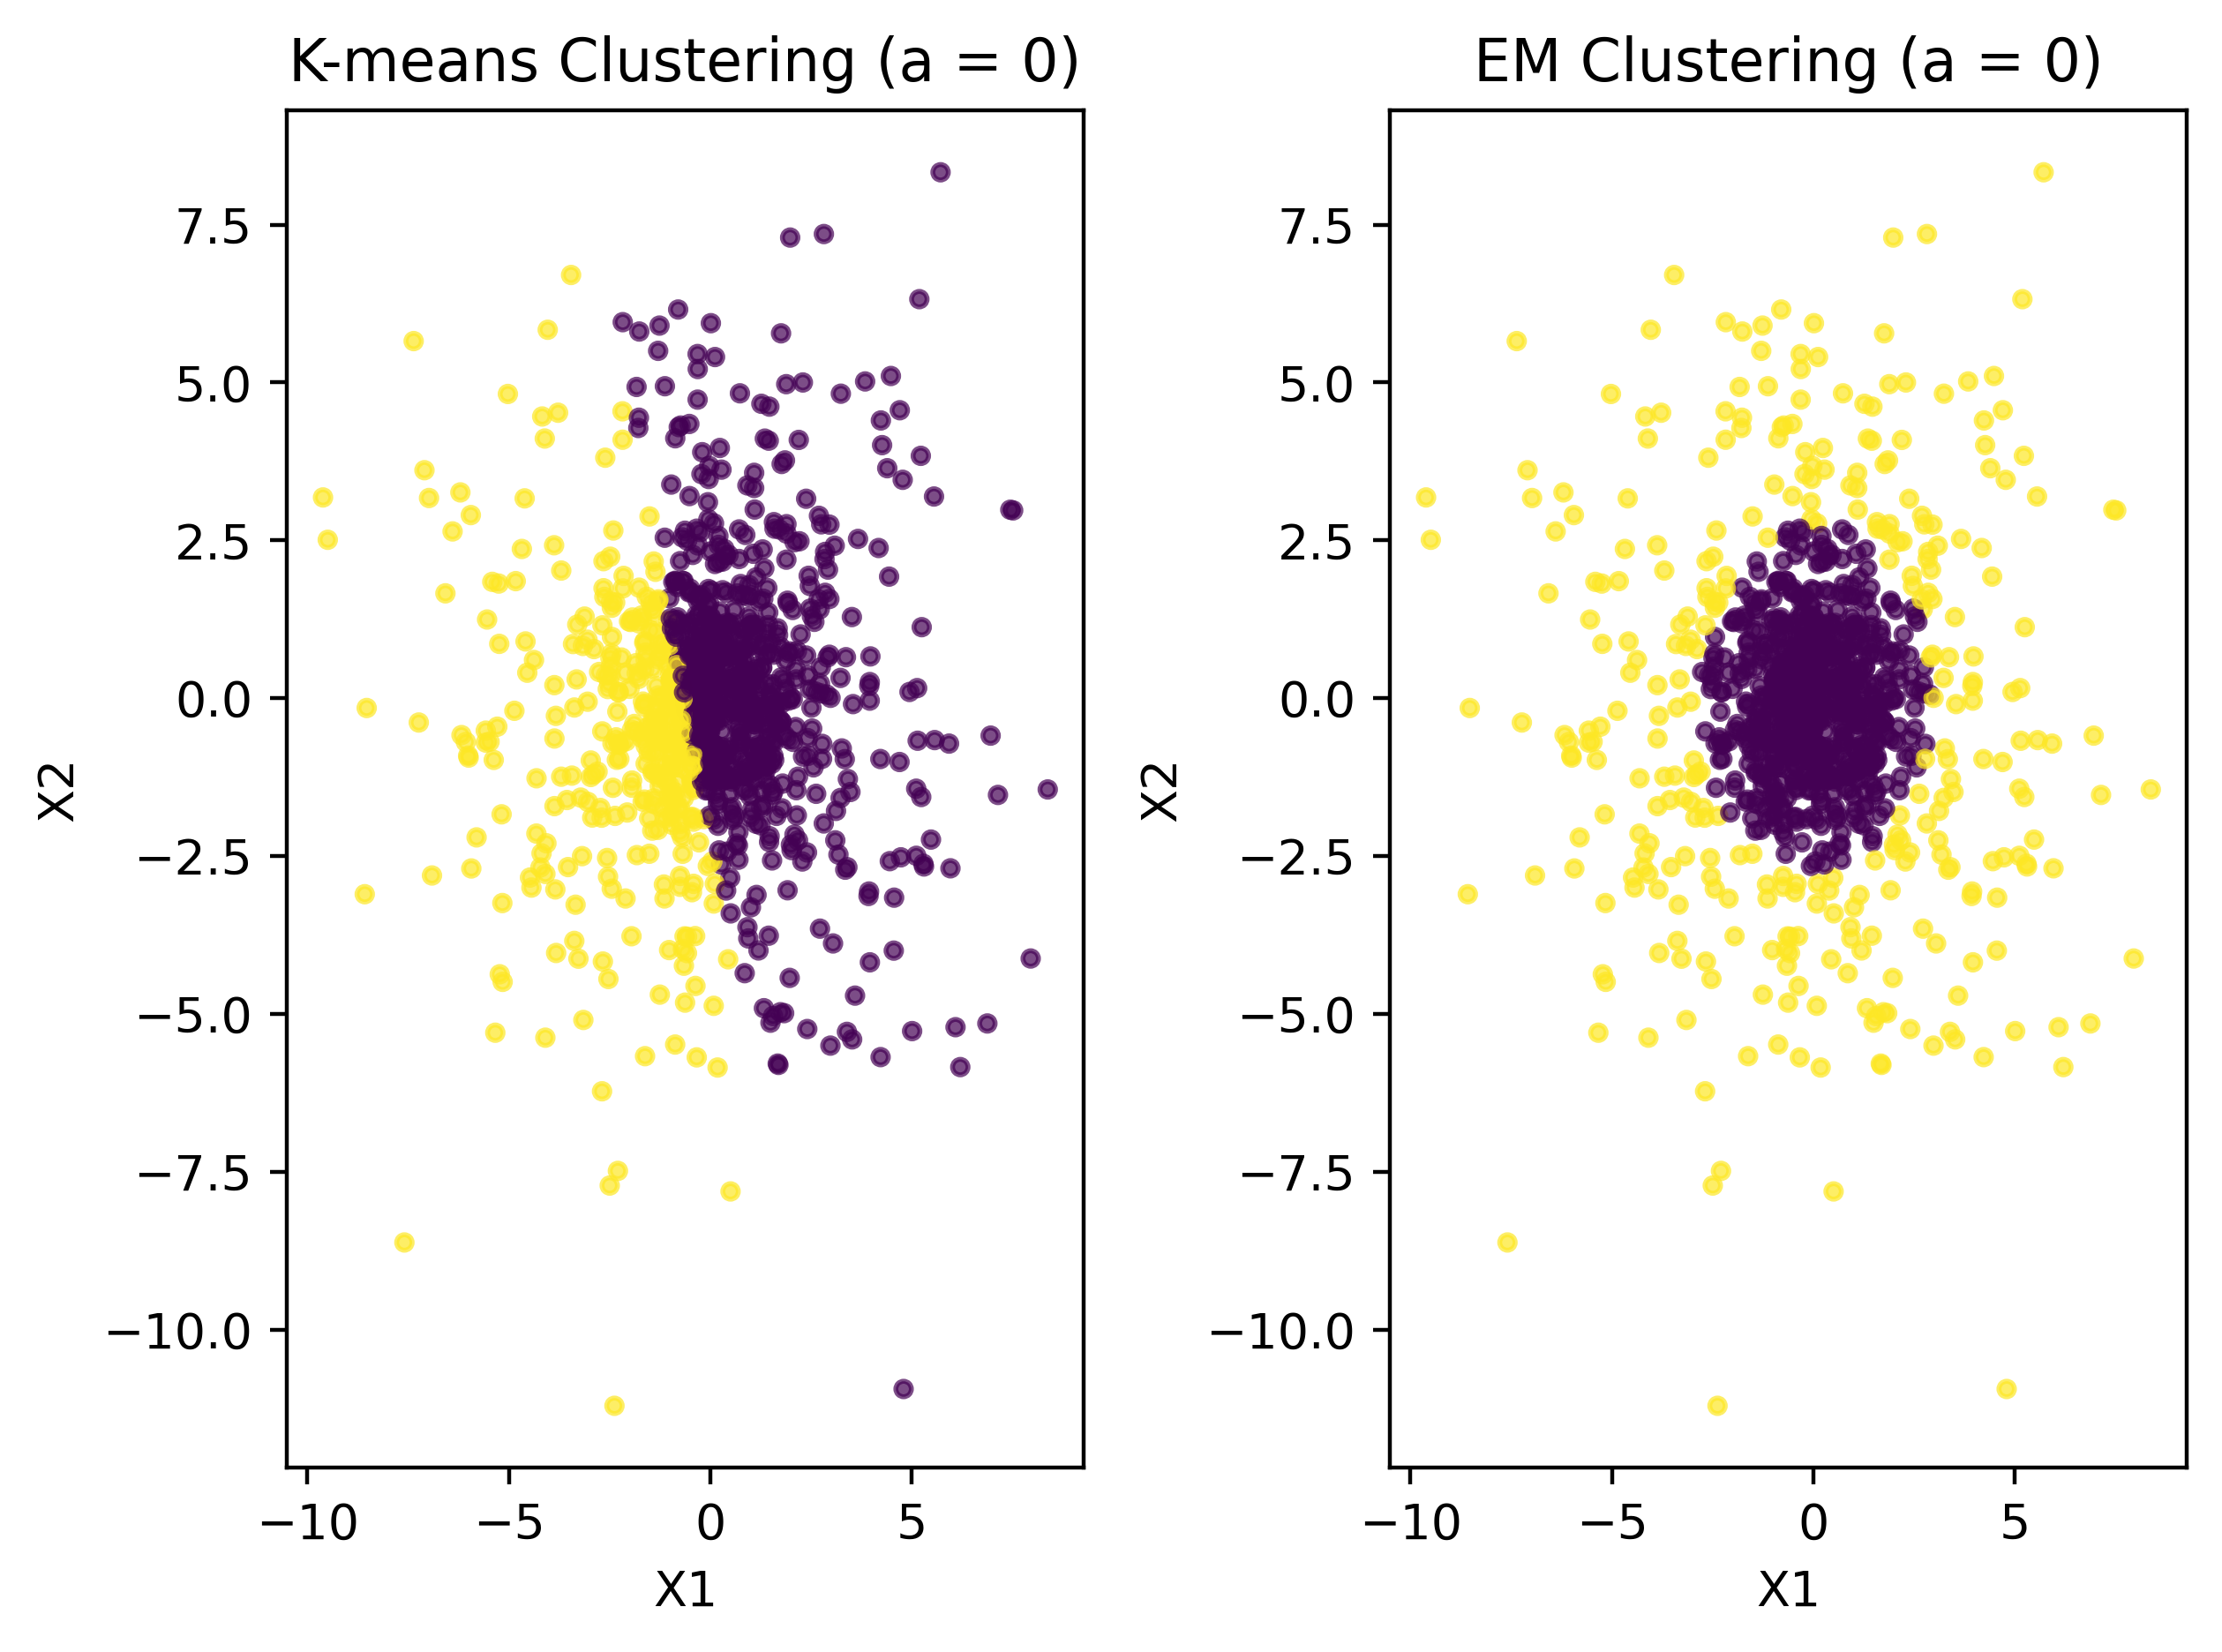
\includegraphics[width=0.5\linewidth]{../figures/cluster_results_a.png} 
    \caption{Clustering Results for K-means and EM, a=0}
\end{figure}

\begin{figure}[htbp]
    \centering 
    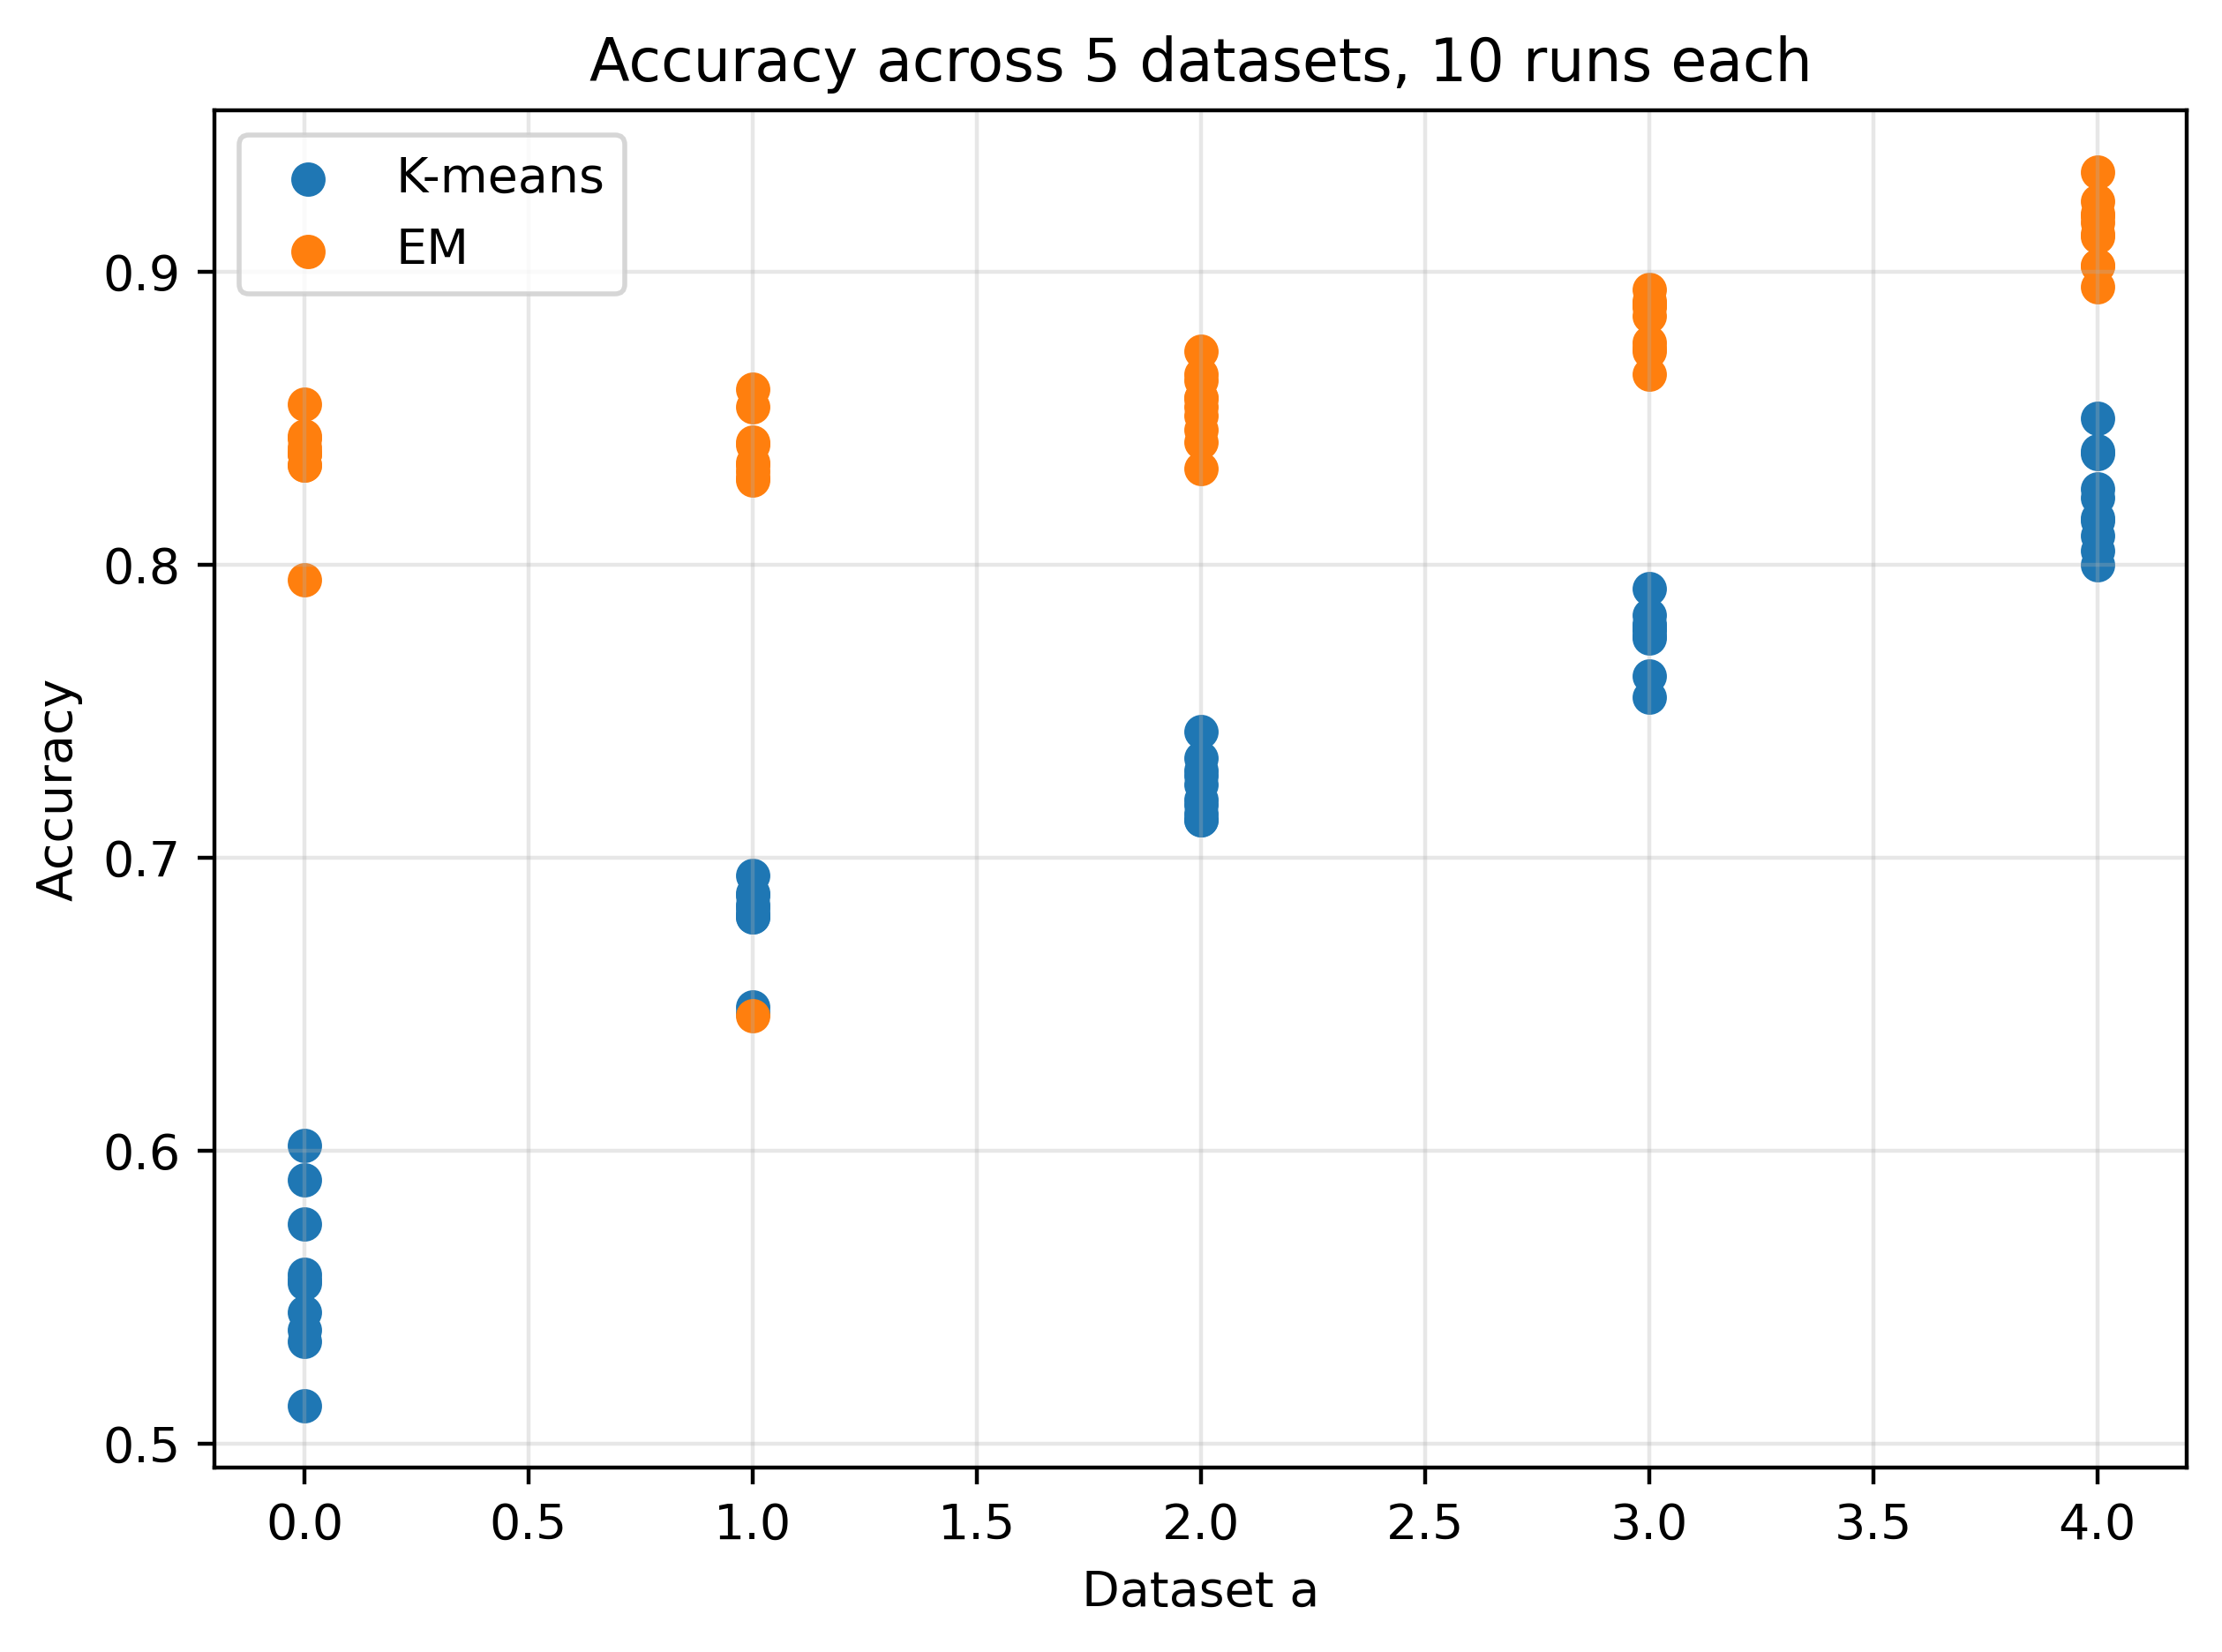
\includegraphics[width=0.5\linewidth]{../figures/accuracy_vs_a.png} 
    \caption{Accuracy for each run vs. dataset parameter a}
\end{figure}

\begin{figure}
    \centering 
    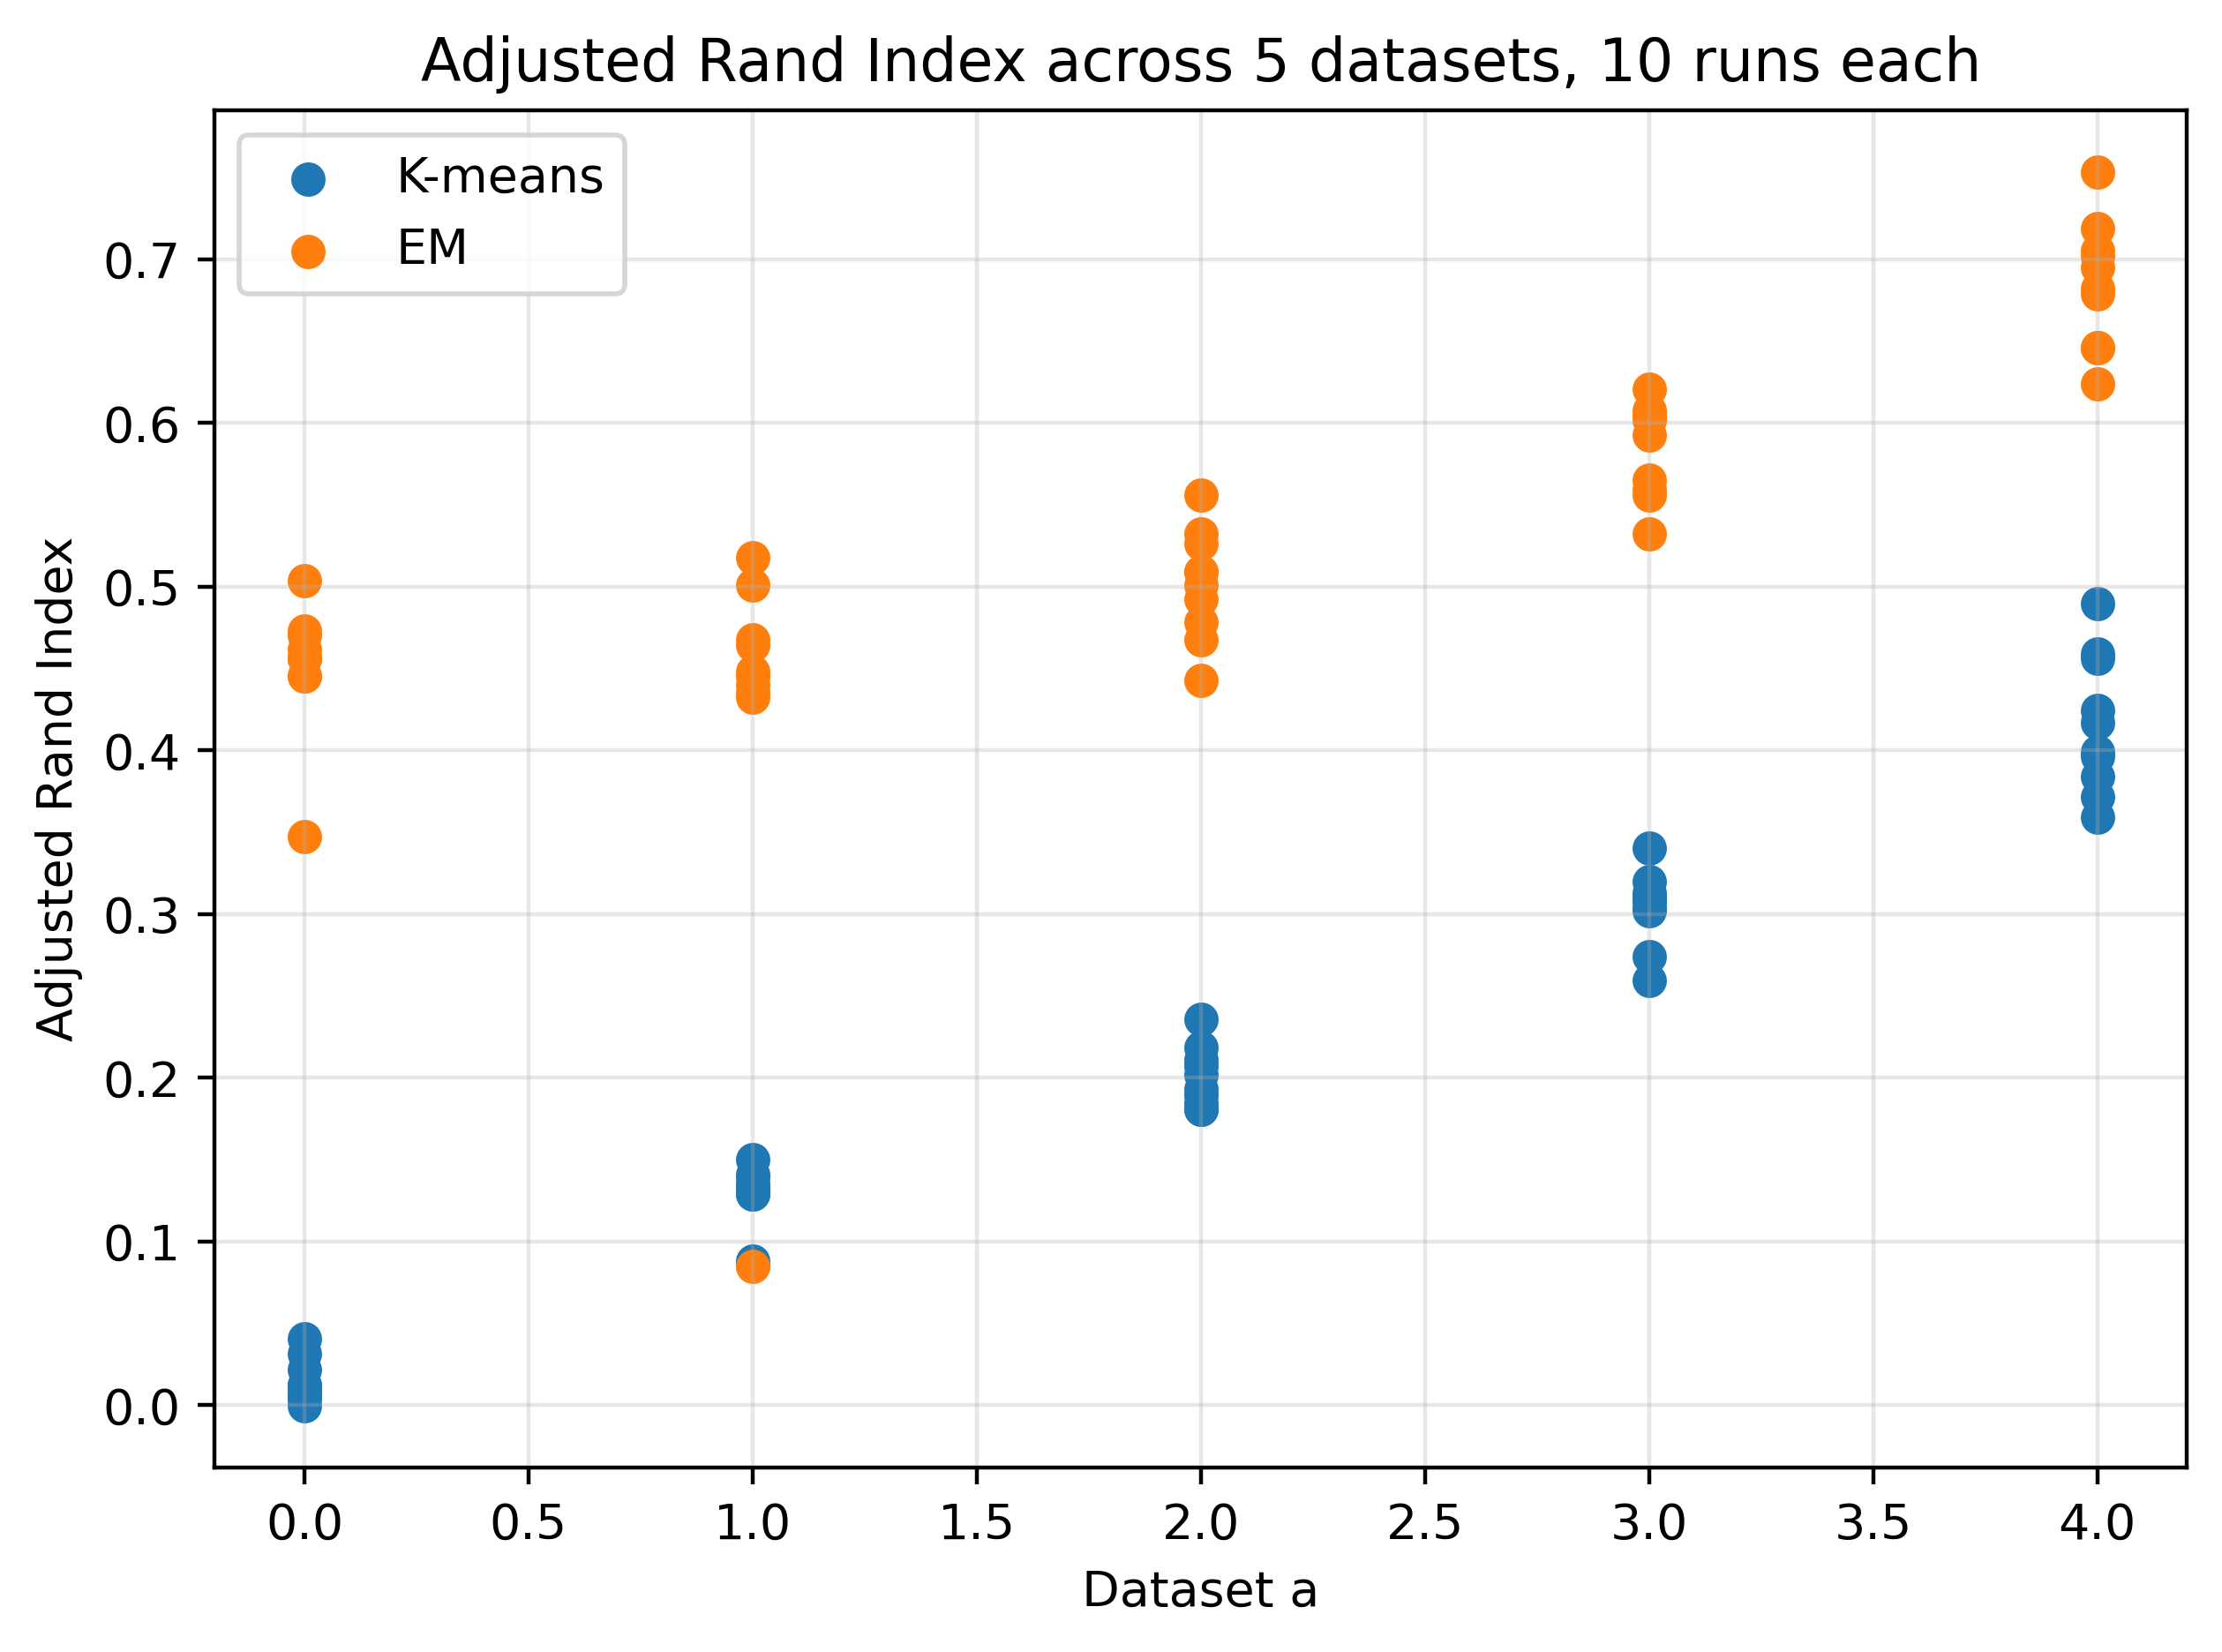
\includegraphics[width=0.5\linewidth]{../figures/ari_vs_a.png} 
    \caption{Adjusted Rank Index for each run vs. dataset parameter a}
\end{figure}

\section*{Part b}

% \newpage
% \newpage
% %adding code
% \appendix
% \section*{Code}
% \lstinputlisting[language=Python]{../code/hw07.py}

\end{document}